\documentclass{article}
\usepackage{polski}
\usepackage{blindtext}
\usepackage{amsmath}
\usepackage{mathtools}
\usepackage{graphicx} 
\usepackage{wrapfig}
\usepackage{amssymb}
\usepackage{multirow}
\usepackage[usenames,dvipsnames,svgnames,table]{xcolor}
\usepackage{float}
\usepackage[caption = false]{subfig}
\usepackage{caption}
\newcommand\tab[1][1cm]{\hspace*{#1}}
\usepackage[a4paper, left=2cm, right=2cm, top=2cm, bottom=2cm, headsep=1.2cm]{geometry}

\usepackage{titling}
\newcommand{\subtitle}[1]{%
  \posttitle{%
    \par\end{center}
    \begin{center}\large#1\end{center}
    \vskip0.5em}%
}


\begin{document}
\title{\textsc{Sprawozdanie - laboratorium 7}}
\subtitle{\textbf{Interpolacja Lagrannge'a z optymalizacją położeń węzłów}}
\author{Zuzanna Grzesik}
\date{15 kwietnia 2020}

\maketitle	

\section{Wstęp teoretyczny}	
\subsection{Interpolacja}
Interpolacja jest to metoda numeryczna, która polega na wyznaczaniu w danym przedziale tzw. funkcji interpolacyjnej $f$, która przyjmuje z góry zadane wartości, w ustalonych punktacji zwanych węzłami. W przedziale $[a, b]$ danych jest $n+1$ różnych punktów $x_0, x_1, ... , x_n$ (węzły) oraz wartości funkcji w tych punktach: $f(x_0) = y_0, f(x_1) = y_1, ... ,f(x_n) = y_n$. Interpolacje najczęściej przeprowadza się korzystając z wielomianów algebraicznych, wielomianów trygonometrycznych lub funkcji sklejanych.
\par Interpolacja wykorzystywana jest do zagęszczania tablic i efektywniejszego rozwiązywania równań nieliniowych dla stablicowanych wartości funkcji z określonymi położeniami węzłów, w postaci wielomianowej do lokalnego przybliżania dowolnych funkcji, co ułatwia rozwiązywanie modeli fizycznych, a także do całkowania numerycznego i modelowania powierzchni w dwóch i trzech wymiarach.
\subsection{Interpolacja Lagrange'a}
Interpolacja Lagrange'a, zwana inaczej wielomianową, jest to rodzaj interpolacji, która do przybliżania funkcji korzysta z wielomianu Lagrange'a postaci:
\begin{equation}
\omega(x) = \displaystyle\sum_{i=0}^{n} y_i \displaystyle\prod_{j=0 \wedge  j \neq i }^{n} \frac{x - x_j}{x_i - x_j},
\end{equation}
gdzie $n$ to stopień wielomianu, dla $n+1$ podanych węzłów.
\subsection{Błędy interpolacji. Dobór węzłów. Efekt Rungego}
Dokładność interpolacji zależy od dobranych do niej węzłów oraz ich ilości. Pozornie wydaje się, że większa liczba węzłów zawsze zwiększa dokładność. W przypadku węzłów równoodległych tak nie jest  - jest to przykład Efektu Rungego. Efekt ten to pogorszenie jakości interpolacji wielomianowej, mimo zwiększenia liczby jej węzłów. Początkowo ze wzrostem liczby węzłów przybliżenie poprawia się, jednak w pewnym momencie zaczyna się ono psuć, co jest szczególnie widoczne na końcach przedziału.\cite{1} Można temu zaradzić, posługując się wielomianami Czebyszewa zamiast węzłami równodległymi.
\subsection{Wielomiany Czebyszewa}
Wielomiany Czebyszewa są określone wzorem:
\begin{equation}
\begin{array}{l}
T_n(x) = \cos[n \cdot arccos(x)], \\
x \in [-1, 1].
\end{array}
\end{equation}
W postaci rekurencyjnej:

\begin{equation}
\begin{array}{l}
T_0(x) = 1\\
T_1(x) = \cos[n \cdot arccos(x)] = x \\
T_n(x) = 2xT_{n-1}(x) - T_{n-2}(x), n \geq 2.
\end{array}
\end{equation}
Z tak zapisanych zależności można wyliczyć zera wielomianów, które są następującej postaci:
\begin{equation}
x_m = cos(\pi \frac{2m +1}{2n + 2}), m=0,1,2, . . . , n.
\end{equation}
Po przeskalowaniu przedziału $[-1, 1]$ na $[a, b]$ otrzymujemy:
\begin{equation}
x_m = \frac{1}{2} [(b -a) cos(\pi \frac{2m +1}{2n + 2}) + (b + a) ]
\end{equation}
Miejsca zerowe wielomianów Czebyszewa zagęszczają się ku krańcom przedziału, co pozwala lepiej związać wielomian zapobiegając naturalnym dla wielomianów wysokiego rzędu oscylacjom. \cite{2}
\section{Zadanie do wykonania}
\subsection{Opis problemu}
Zadaniem w trakcie laboratoriów było znalezienie wielomianu interpolacyjnego Lagrange'a $W_n(x)$, dla funkcji:
\begin{equation}
f(x) = exp(-x^2),
\end{equation}
w przedziale $x \in [-5, 5]$. W tym celu należało napisać program z zaimplementowaną metodą wyznaczającą przybliżone wartość funkcji w położeniu międzywęzłowym wykorzystując wielomianu interpolacyjnego Lagrange'a. Argumentami dla tej funkcji miały być wektor węzłów, wektor wartości funkcji w węzłach, stopień wielomianu (o jeden niższy niż liczba węzłów) oraz wartość $x$ dla której wyliczamy wartość funkcji. 
\par Następnie korzystając z powyższego programu należało przeprowadzić interpolacje funkcji (6) dla  $n = 5, 10, 15, 20$ dla równoodległych węzłów oraz sporządzić wykresy funkcji oraz wielomianu interpolacyjnego na jednym rysunku, dla każdego $n$.
\par Kolejną częścią zadania było zoptymalizowanie położeń węzłów poprzez określenie ich jako zer wielomianów Czebyszewa, określonych wzorem:
\begin{equation}
x_m = \frac{1}{2} [(x_{max} - x_{min}) cos(\pi \frac{2m +1}{2n + 2}) + (x_{max} + x_{min}) ],
\end{equation}
gdzie $m = 0, 1, \cdots, n$, natomiats (n+1) jest całkowitą liczbą węzłów oraz stopnie wielomianu Czebyszewa. Dla tak zoptymalizowanych węzłów należało ponownie przeprowadzić interpolację, dla tych samych wartości co poprzednio, a następnie sporządzić wykresy funkcji $f(x)$ oraz $W_n(x)$.
\subsection{Wyniki}
\begin{figure}[H]
\centering
\subfloat[n = 5, $\Delta x = 2$]{\includegraphics[width=8cm]{inter_n5.eps}}
\subfloat[n = 10, $\Delta x = 1$]{\includegraphics[width=8cm]{inter_n10.eps}}\\
\subfloat[n = 15, $\Delta x = \frac{2}{3}$]{\includegraphics[width=8cm]{inter_n15.eps}}
\subfloat[n = 20, $\Delta x = \frac{1}{2}$]{\includegraphics[width=8cm]{inter_n20.eps}}
\caption{Wyniki interpolacji wielomianem Lagrange'a $W_n(x)$, z równoodległymi węzłami, dla $n+1$ węzłów.}
\end{figure}

Jak widać na powyższych rysunkach, wraz ze wzrostem liczby węzłów wzrasta dokładność obliczonego wielomianu dla wartości w środku przedziału, jednak maleje dokładność dla jego krańców.

\begin{figure}[H]
\centering
\subfloat[n = 5]{\includegraphics[width=8cm]{inter_n5_Czebyszew.eps}}
\subfloat[n = 10]{\includegraphics[width=8cm]{inter_n10_Czebyszew.eps}}\\
\subfloat[n = 15]{\includegraphics[width=8cm]{inter_n15_Czebyszew.eps}}
\subfloat[n = 20]{\includegraphics[width=8cm]{inter_n20_Czebyszew.eps}}

\caption{Wyniki interpolacji wielomianem Lagrange'a $W_n(x)$, z węzłami, których współrzędne są wyznaczone przez miejsca zerowe wielomianów Czebyszewa, dla $n+1$ węzłów.}
\end{figure}

Dla węzłów obliczonych korzystając jako zera wielomianu Czebyszewa, wraz ze wzrostem ilości węzłów wzrasta dokładność interpolacji, na całym przedziale, w przeciwieństwie do węzłów równoodleglych, dla których dokładność ,,psuła się" na krańcach przedziału. 

\section{Wnioski}
Dzięki zwiększaniu liczby węzłów wzrasta dokładność interpolacji, jednak ważnym aspektem jest odpowiedni dobór węzłów. Dla węzłów równoodległych na krańcach przedziału pojawiają się charakterystyczne skoki, które sprawiają, że oszacowanie funkcji nie jest już tak dokładne. Jeżeli jednak dobierzemy węzły korzystając z wielomianów Czebyszewa, które zagęszczają się na krańcach przedziału, możemy dokładniej oszacować postać szukanej funkcji.

\begin{thebibliography}{2}

\bibitem{1}
	\emph{Efekt Rungego} 
  \texttt{https://pl.wikipedia.org/wiki/Efekt\_Rungego}

\bibitem{2}
	\emph{Wielomiany Czebyszewa} 
  \texttt{https://pl.wikipedia.org/wiki/Wielomiany\_Czebyszewa}

\end{thebibliography}

\end{document}
